\documentclass[a4paper,11pt,oneside,onecolumn]{article}
\usepackage[utf8]{inputenc}
\usepackage{cmap}
\usepackage[T1]{fontenc}
\usepackage{beton}
\usepackage{eulervm}
\renewcommand{\sfdefault}{\rmdefault}
\usepackage[pdftex,colorlinks,citecolor=black,filecolor=black,linkcolor=black,urlcolor=black]{hyperref}
\usepackage{tikz}
\usetikzlibrary{positioning,arrows,automata,decorations.pathreplacing,decorations.text,decorations.markings,arrows,shapes,calc,fit}
\usepackage{caption}
\usepackage{subcaption}
\usepackage{multirow}
\usepackage{hhline}
\usepackage{graphicx}
\usepackage{amsmath}
\usepackage[noend]{algpseudocode}

\title{Homework 2}
\author{Mitar Milutinovic (24090156)\thanks{Worked together with Daniel Aranki, Shiry Ginosar, Valkyrie Savage, Orianna DeMasi.}}

\renewcommand\thesection{\arabic{section}.}
\renewcommand\thesubsection{\thesection (\alph{subsection})}

\begin{document}

\maketitle

\section{}

\subsection{}

\begin{center}
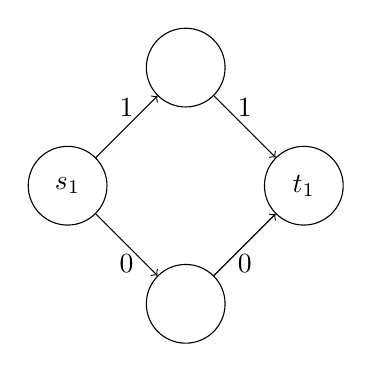
\begin{tikzpicture}

\node[draw,circle,minimum size=1cm] (s) at (0,0) {$s_1$};
\node[draw,circle,minimum size=1cm] (t) at (3,0) {$t_1$};
\node[draw,circle,minimum size=1cm] (n1) at (1.5,1.5) {};
\node[draw,circle,minimum size=1cm] (n2) at (1.5,-1.5) {};
\draw[->] (s) -- node[above] {$1$} (n1);
\draw[->] (n1) -- node[above] {$1$} (t);
\draw[->] (s) -- node[below] {$0$} (n2);
\draw[->] (n2) -- node[below] {$0$} (t);

\end{tikzpicture}
\end{center}

Path routing from $s_1$ to $t_1$ has congestion equal to $1$ (two possible paths are mirrored).

\begin{center}
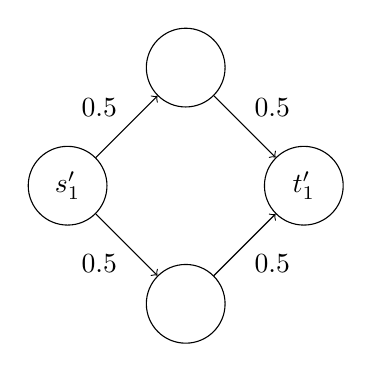
\begin{tikzpicture}

\node[draw,circle,minimum size=1cm] (s) at (0,0) {$s_1'$};
\node[draw,circle,minimum size=1cm] (t) at (3,0) {$t_1'$};
\node[draw,circle,minimum size=1cm] (n1) at (1.5,1.5) {};
\node[draw,circle,minimum size=1cm] (n2) at (1.5,-1.5) {};
\draw[->] (s) -- node[above left] {$0.5$} (n1);
\draw[->] (n1) -- node[above right] {$0.5$} (t);
\draw[->] (s) -- node[below left] {$0.5$} (n2);
\draw[->] (n2) -- node[below right] {$0.5$} (t);

\end{tikzpicture}
\end{center}

Fractional path routing from $s_1'$ to $t_1'$ has congestion equal to $0.5$.

\subsection{}

$p_i$ is a set of all paths $p_{i_j}$ that connect $s_i$ and $t_i$.
Length of path $p_{i_j}$ is $d(p_{i_j})$. Each path $p_{i_j}$ routes a fraction $f(p_{i_j})$ of common
$f(p_{i}) = 1$, unit flow.
$c(e)$ is congestion on edge $e$ under routing,
which is in our case sum of all fractional flows of all paths across edge $e$.

\begin{align*}
\max_e c(e) & \ge \sum_e d(e) c(e) \\
 & = \sum_e d(e) \sum_i \sum_{j:p_{i_j} \ni e} f(p_{i_j}) \\
 & = \sum_e \sum_i \sum_{j:p_{i_j} \ni e} f(p_{i_j}) d(e) \\
 & = \sum_i \sum_j \sum_{e \in p_{i_j}} f(p_{i_j}) d(e) \\
 & = \sum_i \sum_j f(p_{i_j}) \sum_{e \in p_{i_j}} d(e) \\
 & = \sum_i \sum_j f(p_{i_j}) d(p_{i_j}) \\
 & \ge \sum_i 1 \cdot \min_j d(p_{i_j}) \\
 & = \sum_i d(s_i, t_i) \\
\end{align*}

\setcounter{section}{2}

\section{}

\subsection{}

If after increasing the weight for $\delta$ on edge $(u, v)$ cover is still feasible, we do not have to do anything. Otherwise,
we start to repeatedly adjust the $p$. We maintain the priority queue $Q$ of edges with the most infeasible edge at the front.
We set $p(v) \gets p(v) + \delta$ and add all other edges connected to $v$ to $Q$. From $Q$ we pop one edge $(u', v')$ (the currently most
infeasible edge) and compute new $\delta \gets w(u', v') - p(u') - p(v')$. We set $p(u') \gets p(u') - \delta$ and repeat the process
of adjusting on $u'$. We repeat until $\delta$ becomes $0$.

\subsection{}

Algorithm si $O(m \log n)$, processing $m$ edges in the graph in the priority queue order.

\end{document}
